\chapter[GDPR Documentation and Ethical Approval]{GDPR Documentation and\\Ethical Approval} % Square brackets is for TOC. Curly brackets for actual page.

%\epigraph{\flushleft --- Do you know a good \textsc{GDPR} consultant?\\ --- Yes.\\ --- Can you pass me their email address?\\ --- No.}

This research project discharges its duty imposed by the \textsc{EEA}'s general data protection regulation (\textsc{GDPR}) by following Norwegian Centre for Research Data (\textsc{NSD})'s \href{https://nsd.no/personvernombud/en/notify/notification_test.html}{notification test} on Friday, 11 September 2020. Both \href{https://www.oecd.org/pisa/data/2018database/}{\textsc{PISA} 2018 Database} and the \href{https://data.worldbank.org/}{World Bank Open Data} contain only aggregated and de-personalised datasets with no possibility of back-tracing to any particular participant. Resultantly, no identifiable personal data were collected or used at any stage of this research. The \textsc{NSD}'s assessment letter outlines the agency's decision of not subjecting this project to the \textsc{GDPR} notification. The \textsc{NSD} decision letter also satisfies University of Oslo's \href{https://www.uio.no/english/for-employees/support/research/funding/units/hf/imv/data-ethics/}{ethical approval requirement} and concludes the approval process.

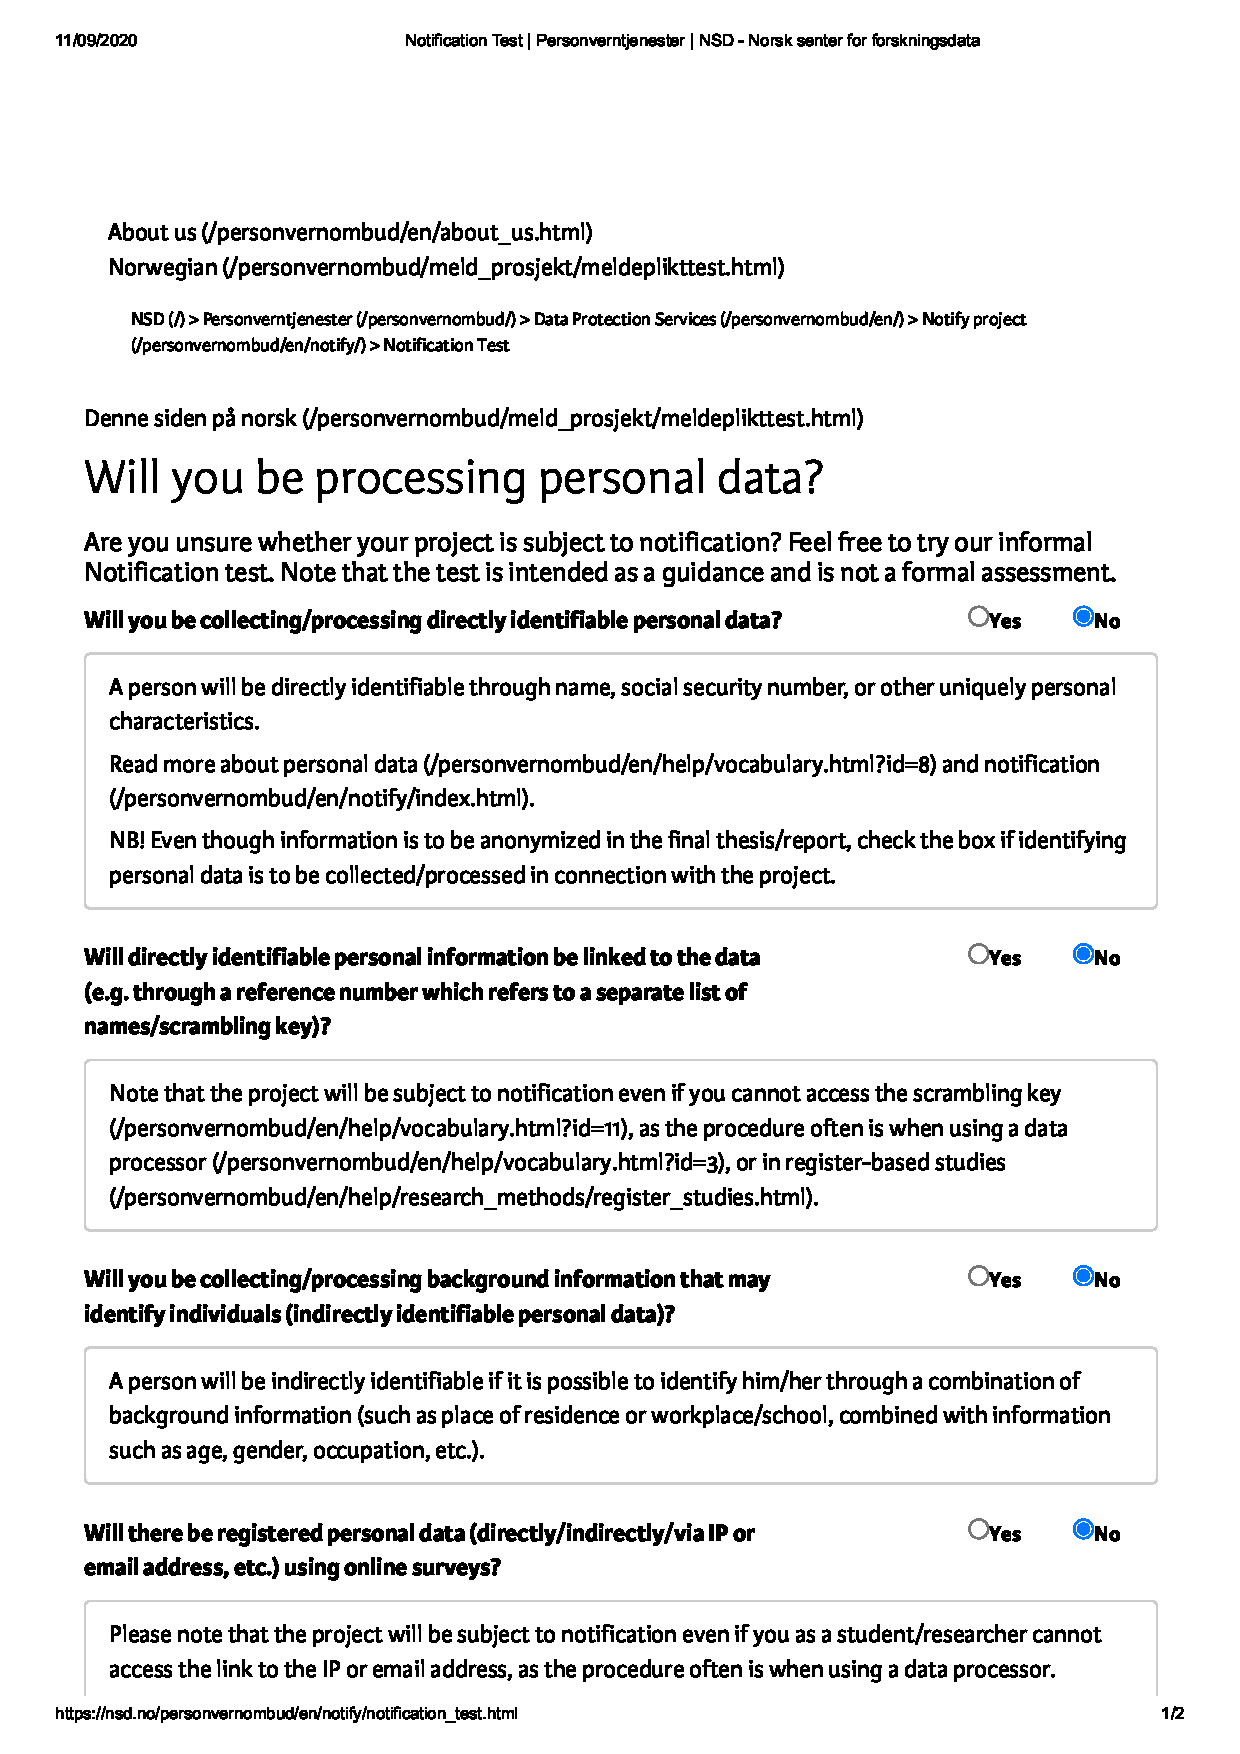
\includepdf[pages=-,fitpaper=true,noautoscale=true]{Appendices/Notification-Test.pdf}

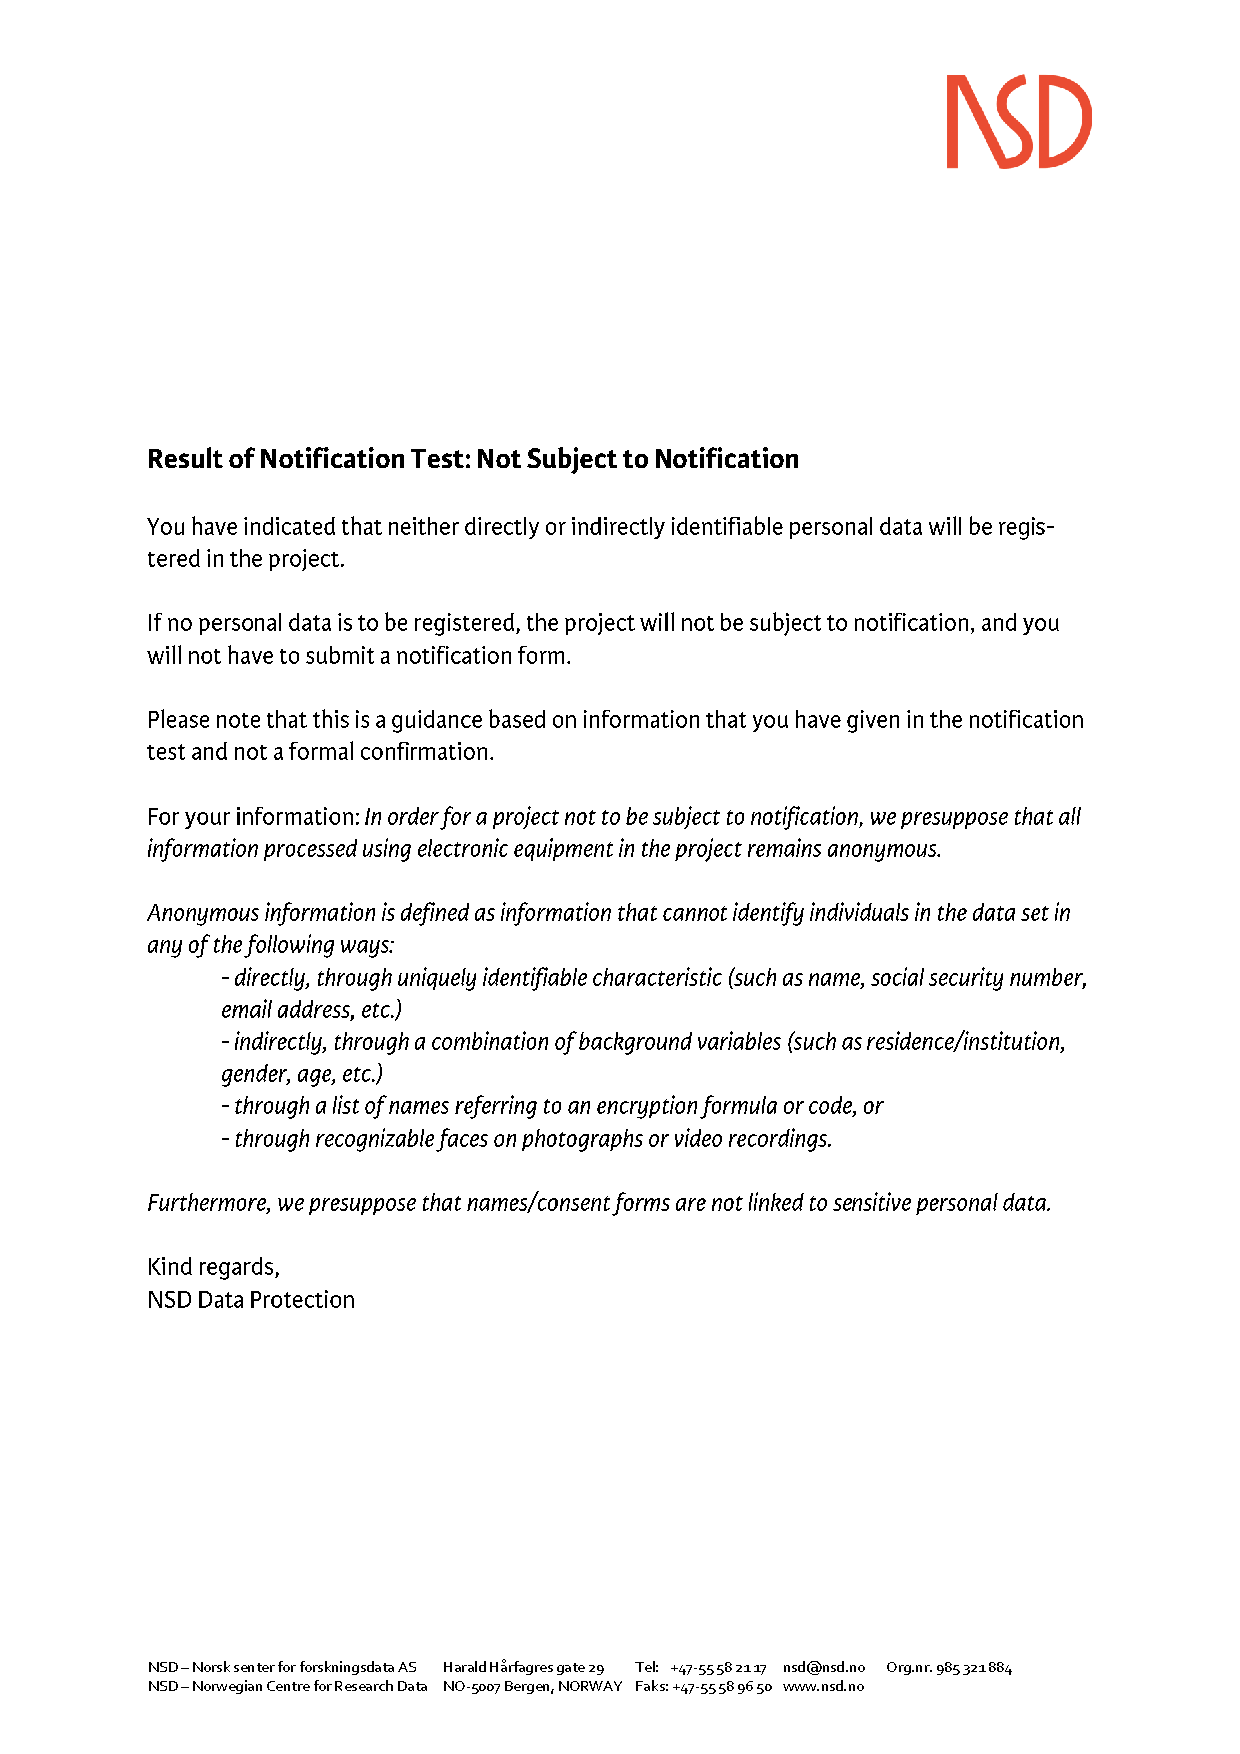
\includepdf[pages=-,fitpaper=true,noautoscale=true]{Appendices/not_subject_to_notification.pdf}

